\documentclass[12pt, twoside]{article}
% \documentclass[12pt, twoside]{article}
\usepackage[letterpaper, margin=1in, headsep=0.2in]{geometry}
\setlength{\headheight}{0.6in}
%\usepackage[english]{babel}
\usepackage[utf8]{inputenc}
\usepackage{microtype}
\usepackage{amsmath}
\usepackage{amssymb}
%\usepackage{amsfonts}
\usepackage[nomessages]{fp} %\FPeval{\var-name}{2*sin(pi/6)}
\usepackage{siunitx} %units in math. eg 20\milli\meter
\usepackage{yhmath} % for arcs, overparenth command
\usepackage{tikz} %graphics
\usetikzlibrary{quotes, angles, arrows, arrows.meta}
\usepackage{graphicx} %consider setting \graphicspath{{images/}}
\usepackage{parskip} %no paragraph indent
\usepackage{enumitem}
\usepackage{multicol}
\usepackage{venndiagram}

\usepackage{fancyhdr}
\pagestyle{fancy}
\fancyhf{}
\renewcommand{\headrulewidth}{0pt} % disable the underline of the header
\raggedbottom
\hfuzz=2mm %suppresses overfull box warnings

\usepackage{hyperref}
\usepackage{float}

\fancyhead[LE]{\thepage}
\fancyhead[RO]{\thepage \\ First and last name: \hspace{2.5cm} \,\\ Section: \hspace{2.5cm} \,}
\fancyhead[LO]{BECA / Dr. Huson / Regents Prep: Graphs\\* 2 December 2024}

\begin{document}

\subsubsection*{1.14 Do Now: Graphing inequalities}
\begin{enumerate}
  \item Graph and label the two inequalities on the grid. 

  \begin{multicols}{2}
    $\displaystyle y \geq 2x-2$ \\
    $x+ \frac{1}{2}y < 3$
    \end{multicols} \vspace{1cm}

  \begin{center} %4 quadrant regents grid w T-Chart
  \begin{tikzpicture}[scale=.635]
    \draw [help lines] (-10,-10) grid (10,10);
    \draw [thick, ->] (-10.2,0) -- (10.4,0) node [below right] {$x$};
    \draw [thick, ->] (0,-10.2)--(0,10.4) node [left] {$y$};
  \end{tikzpicture}
  \end{center}

Mark a point in the solution set and label it with the ordered pair.

\newpage
\item Slide $\triangle ABC$ to the right three and up four. Label the image $\triangle A'B'C'$.
\begin{center}
    \begin{tikzpicture}[scale=.55]
    \draw [help lines] (-7,-3) grid (10,6);
    \draw [thick, <->] (-7.4,0) -- (10.4,0) node [right] {$x$};
    \draw [thick, <->] (0,-3.4)--(0,6.4) node [above] {$y$};  
    \draw [thick]
      (-1,-1) node[below left] {$A$}--
      (5,-2) node[below] {$B$}--
      (2,1) node[above right] {$C$}--cycle;  
  \end{tikzpicture}
\end{center}

\item In the diagram below, $\triangle ABC$ with sides of 13, 15, and 16, is mapped onto $\triangle DEF$ after a clockwise rotation of $90^\circ$ about point $P$. 
  \begin{multicols}{2}
    \begin{enumerate}
      \item What is $A$ mapped to? $A \rightarrow$ \vspace{0.5cm}
      \item What corresponds to $F$? \vspace{0.5cm}
      \item Given $DF=3x+1$. Find $x$. \\[1.5cm] \;
    \end{enumerate}
    \begin{tikzpicture}[scale=.6, rotate=-30]
      %\draw [thick, <->] (-7.4,0) -- (10.4,0) node [right] {$x$};
      %draw [thick, <->] (0,-5.4)--(0,10.4) node [above] {$y$};
      \fill (0,0) circle[radius=0.1] node[right]{$P$};
      \draw [thick]
        (-2,1) node[below left] {$A$}--
        (-7,2) node[left] {$B$}--
        (-4,5) node[above right] {$C$}--cycle;
        \node at (-5,1.5)[below]{16};
        \node at (-6,4){13};
        \node at (-2.5,3.5){15};
        \node at (3.25,2.25){$3x+1$};
      \draw [thick]
        (1,2) node[left] {$D$}--
        (2,7) node[above] {$E$}--
        (5,4) node[right] {$F$}--cycle;
    \end{tikzpicture}
  \end{multicols}

\item On the axes below, graph the point $P(2,4)$ and its image, $P'$, after a rotation of $90^\circ$ counterclockwise around the origin. Label both points as a coordinate pair.
    \begin{center}
      \begin{tikzpicture}[scale=.6]
      \draw [help lines] (-5,-5) grid (5,5);
      \draw [thick, <->] (-5.4,0) -- (5.4,0) node [right] {$x$};
      \draw [thick, <->] (0,-5.4)--(0,5.4) node [above] {$y$};
      \foreach \x in {-5,...,-2,1,2,3,4,5}
        \draw[shift={(\x,0)},color=black] (0pt,-3pt) -- (0pt,3pt) node[below=5pt]  {$\x$};
      \foreach \y in {-5,...,-1,1,2,3,4,5}
        \draw[shift={(0,\y)},color=black] (-3pt,0pt) -- (3pt,0pt) node[left=5pt]  {$\y$}; 
    \end{tikzpicture}
  \end{center}

\end{enumerate}
\end{document}